\documentclass[11pt]{article}

\usepackage{epsilonj}

\RequirePackage{graphicx}
\RequirePackage[colorlinks,citecolor=blue,urlcolor=blue]{hyperref}

\usepackage{colortbl}
\definecolor{rrow}{rgb}{1,0.9,1}
\definecolor{ccol}{rgb}{1,1,0.6}
\definecolor{inters}{rgb}{1,0.9,0.6}

\usepackage{amsmath}
\usepackage{xfrac}
\usepackage{multirow}
\usepackage{tablefootnote}

\addbibresource{../../template/epsilon.bib}

\begin{document}
\setcounter{page}{15}

\TITLE{Измерение и наглядное представление практической значимости регрессионных связей}
\SHORTTITLE{Измерение и наглядное представление практической значимости регрессионных связей}
		
\AUTHOR{Кирилл Фурманов}{Кафедра математической экономики и~эконометрики, НИУ ВШЭ, Москва.}
\SHORTAUTHOR{Фурманов К. К.}
		
\DoFirstPageTechnicalStuff
		
\begin{abstract}

\end{abstract}
		
\begin{keyword}

\end{keyword}
 


{\it «Over time we learn about and use fancier and more abstract regression models… The utility of these fancier models diminishes if we have greater difficulty interpreting and visualizing the results»}\footnote{Michael N. Mitchell. Interpreting and Visualizing Regression Models Using Stata. Stata Press, 2012.}

\bigskip
Среди экономических исследований значительную долю составляют работы, направленные на определение детерминант какой"=либо интересующей исследователя величины (заработной платы, продолжительности периода безработицы и~т.п.). Основным инструментом анализа в~таких случаях оказывается, как правило, модель множественной регрессии. Интерпретация результатов регрессионного анализа сводится, по большей части, к~двум аспектам: истолкованию оценок коэффициентов регрессии и~их статистической значимости. Во многих моделях (особенно нелинейных) оценки с~трудом поддаются интерпретации, что побуждает обращаться к~дополнительным средствам: расчёту предельных эффектов, сравнению прогнозных значений объясняемой переменной при различных значениях детерминант, построению графиков функции отклика. Однако функции отклика "--- характеристика исключительно динамических моделей, а~предельные эффекты и~различия в~прогнозах зависят от того, при каких уровнях объясняющих переменных их рассчитывать. Результаты таких расчётов сложно систематизировать, свести в~одну ясную картину связи переменной отклика с~регрессорами, так что основная цель моделирования "--- сведение большого объёма информации к~небольшому числу интерпретируемых параметров "--- не достигается. Что касается значимости оценок, то значительное число недоразумений и~вольных истолкований (среди них "--- подмена статистической значимостью практической важности) позволяют утверждать, что неверная интерпретация статистической значимости "--- одна из наиболее распространённых ошибок в~статистике (Good, Hardin, 2012). В действительности, применение аппарата проверки статистических гипотез даёт весьма скудную информацию о практической важности связи по многим причинам: 

\begin{itemize}
	\item <<однобокость» вывода (можно обнаружить связь, но не её отсутствие), 
	\item невозможность ранжировки объясняющих переменных по значимости их вклада, 
	\item возможность высокой статистической значимости совершенно незначительных с~практической точки зрения коэффициентов,
	\item сомнительная применимость вероятностных методов к не экспериментальным данным.
\end{itemize}

В~этой статье я~попытаюсь показать, как можно дополнить традиционные способы представления оценок регрессионных моделей и~приблизить исследователя к~оцениванию практической значимости статистических связей. Конечно, практическую значимость невозможно формализовать "--- в каждой реальной задаче есть свои особенности, определяющие важность модельных коэффициентов. Можно лишь снабдить исследователя набором способов представления данных и~сведения их к~небольшому количеству осмысленных параметров, которые помогли бы ему самому оценить значительность выявленных связей. Здесь я~ограничусь измерением вклада объясняющих переменных в~разброс отклика, то есть рассмотрю способы ответить на вопрос: в~какой мере различия между наблюдениями в величине отклика могут быть связаны со значениями некоторого регрессора.

Прежде чем перейти к~сути, рассмотрим ещё одну опасность в~интерпретации статистических оценок "--- подмену практической важности связи её теснотой. Рисунок~\ref{fig:regression} даёт пример связи тесной, при которой одна из величин почти не изменяется при изменении другой (чёрные кружки, линия регрессии со слабым наклоном), и~пример связи куда менее тесной, при которой, однако, средний уровень одной из величин заметно зависит от значений другой (квадраты с белой заливкой, линия регрессии с~большим наклоном).

\begin{figure}[htbp]
	\centering
	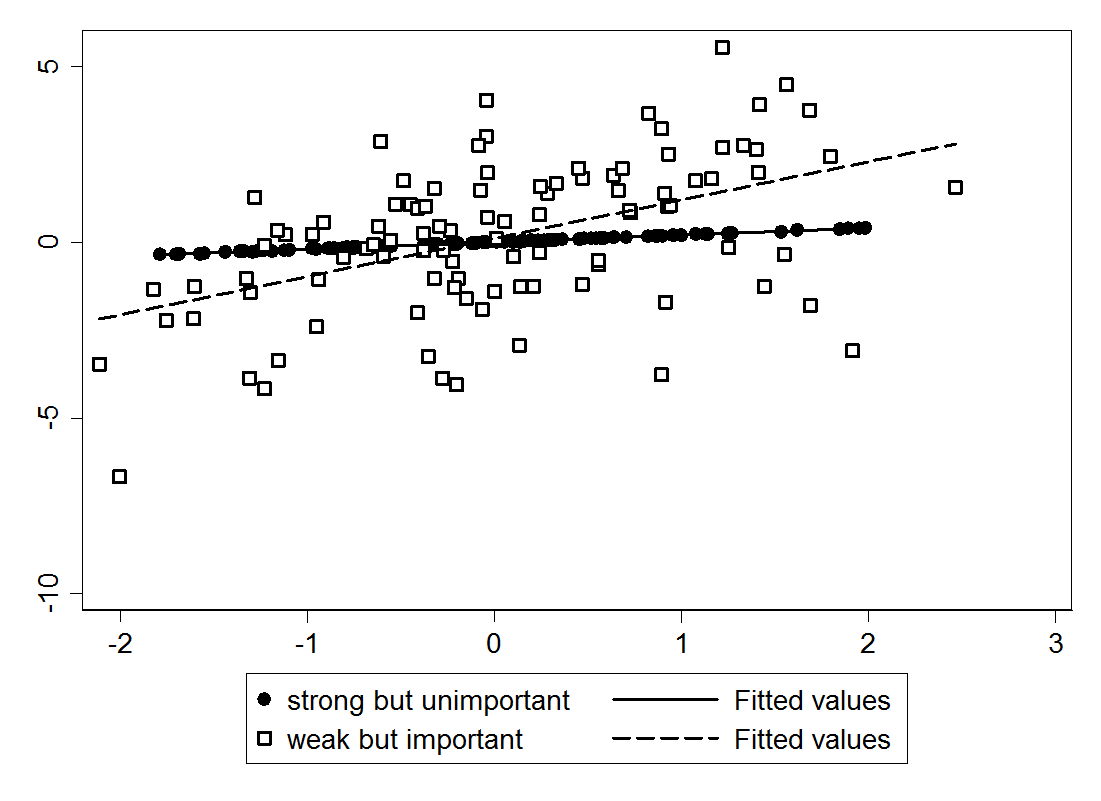
\includegraphics[width=12cm]{regression.png}
	\caption{Название рисунка}\label{fig:regression}
\end{figure} 


После рассмотрения этого рисунка может возникнут мысль, что практическую значимость отражает величина коэффициента регрессии, однако обратим внимание на два факта:
\begin{itemize}
	\item Коэффициент регрессии зависит от единиц измерения регрессора.	Всегда можно подобрать такие единицы измерения, чтобы какой-либо регрессор имел наибольший коэффициент и, таким образом, представлялся самым важным. Единицы измерения отклика тоже играют роль, но не мешают сравнению вклада объясняющих переменных. Хотя, пожалуй, стоит сделать уточнение: сравнивая два облака на рисунке, мы предполагаем, что речь идёт о~связи одних и~тех же статистических признаков, единицы измерения которых для обоих случаев совпадают.
	\item Большой коэффициент может стоять при почти не варьирующемся признаке, так что вклад этого признака в разброс объясняемой величины будет невелик.
\end{itemize}

Решение этих проблем известно: чтобы ранжировать регрессоры по уровню важности их вклада в~разброс объясняемой переменной можно рассчитать стандартизованные коэффициенты регрессии\footnote{Существует множество других мер относительной важности, которые изложены в~обзорах (Kruskal, 1984), (Nathans et al., 2012), (Johnson, LeBreton,  2004), (Soofi, 2000), но они, по большей части, основаны скорее на измерении тесноты связи, способности объясняющей переменной снизить необъяснённую часть разброса отклика.}\fnnsp.
Стандартизованный коэффициент (иногда используется термин «бета-коэффициент») определяется так:

\[\beta_j^* = \beta_j\frac{\sigma_{x_j}}{\sigma_y} \]

Умножение на стандартное отклонение соответствующего регрессора и~деление на стандартное отклонение отклика приводят к~тому, что стандартизованный коэффициент не зависит от единиц измерения переменных модели. Кроме того, если коэффициенты при двух объясняющих переменных совпадают, стандартизованный коэффициент окажется больше у регрессора с большей дисперсией.

Интересный факт: стандартизованные коэффициенты почти игнорируются экономистами. О~частоте использования каждый может получить представление сам, зайдя, например, на сайт \url{repec.org} и запустив поиск словосочетания «standardized coefficients» или «standardized regression coefficients». Современные учебники по эконометрике Грина, Вербика, Баума, Камерона и~Триведи либо не уделяют внимания стандартизованным коэффициентам, либо упоминают о~них вкратце как о~способе получить оценки, не зависящие от единиц измерения. Это замечание не относится к~книгам по неэкономическим приложениям статистических методов, а~также к~учебнику (Johnston, DiNardo, 1997).

Хотя стандартизация полезна при изучении практической значимости регрессоров, потому что позволяет сравнивать их вклад в~разброс объясняемого признака, стандартизованные коэффициенты всё же имеют существенные недостатки:
\begin{itemize}
	\item Их неудобно интерпретировать. Мы можем сказать, что увеличение регрессора $x_j$ на одно стандартное отклонение сопряжено с~ожидаемым увеличением объясняемой величины на $\beta_j^*$ стандартных отклонений при прочих равных условиях.	Это толкование вряд ли удовлетворительно, потому что стандартное отклонение "--- неудобная для интерпретации характеристика.
	\item Нормировка на $\sigma_i$ имеет нежелательный эффект: большой стандартизованный коэффициент может наблюдаться в~случае, когда объясняемая переменная почти не варьируется при изменении регрессора. С~практической точки зрения нам скорее важно оценивать изменение отклика в~натуральных единицах.
\end{itemize}

Второй недостаток легко решаем: достаточно перейти к~полустандартизованным (semistandardized) коэффициентам $\beta_j^{**} = \beta_j\sigma_{x_j}$, однако проблема неинтерпретируемости остаётся. Так как проблема эта вызвана недостатком стандартного отклонения как меры разброса, разумным решением будет использование другой меры. Отдадим предпочтение мерам, основанным на квантилях "--- квантильному размаху (разности двух квантилей случайной величины) и~квантильному коэффициенту (отношению двух квантилей). Переход к~квантильным мерам "--- не единственный способ превратить полустандартизованный коэффициент в~нечто интерпретируемое, но именно этот способ будет удобен нам для графического представления.

\subsection*{Измерение вклада объясняющей переменной в случае линейной зависимости}

Рассмотрим линейное уравнение $y = \beta_1 + \beta_2x_2 + \beta_3x_3 + \ldots + \beta_kx_k + \epsilon$. 
Обозначим за $\mathcal{Q}_j(p)$ функцию квантилей\footnote{Точнее, выборочную функцию квантилей. В~дальнейшем везде речь идёт именно о~выборочных характеристиках.} регрессора $x_j$. Квантильный размах порядка $\gamma$ равен $\mathcal{Q}_j\left(\frac{1+\gamma}{2}\right)-\mathcal{Q}_j\left(\frac{1-\gamma}{2}\right)$ "--- это длина отрезка, включающего долю $\gamma$ всех наблюдений за величиной $x_j$. Домножив эту величину на коэффициент $\beta_j$, получаем удобную характеристику важности объясняющей переменной:
\[CS_j = \beta_j\left(\mathcal{Q}_j\left(\frac{1+\gamma}{2}\right)-\mathcal{Q}_j\left(\frac{1-\gamma}{2}\right)\right)\]

Буквы $CS$ "--- аббревиатура для contribution spread (размах вклада). Интерпретация: если бы наблюдения в~нашей выборке отличались только значениями регрессора $x_j$, а~остальные объясняющие переменные и~случайная ошибка не менялись бы от наблюдения к~наблюдению, то, согласно нашей модели, квантильный размах значений объясняемой величины составил бы $CS_j$ единиц. Иначе говоря, в~средних $\gamma \times 100\%$ наблюдений наибольшее различие между величиной отклика составило бы $CS_j$. 

Наиболее ясной такая интерпретация выглядит при использовании полного размаха "--- разности между наибольшим и~наименьшим значением признака, но 100\% размах чувствителен к~выбросам. Кроме того, использование 100\% размаха создаёт проблемы при распространении результатов на генеральную совокупность: наиболее часто применяемые вероятностные распределения имеют бесконечный размах. Поэтому разумнее сосредоточиться на центральных 90\% или 95\% наблюдений или любой другой доле по желанию исследователя.

\subsubsection*{{\it Пример 1. Модель участия женщин в~рабочей силе}}

По данным о 50 штатах США\footnote{Взяты из книги (Newbold, 2007)} оценивалось уравнение:
\[LFP_i = \beta_1 + \beta_2Income_i + \beta_3Educ_i + \beta_4UR_i + \epsilon_i,\]
где $LFP_i$ "---  уровень участия женщин в~рабочей силе в~штате $i$ (\%),

$Income_i$ "--- медианный доход домохозяйства (тыс. долл.),

$Educ_i$ "--- средняя продолжительность обучения среди женщин (годы),

$UR_i$ "--- уровень безработицы среди женщин (\%).

\medskip
Таблица ниже содержит оценки коэффициентов и~важности вклада каждого из объясняющих признаков:

\begin{table}[h]
	\centering
	\begin{tabular}{|l|c|c|c|c|}
		\hline {\it признак} & {\it коэффициент} & {\it станд. коэфф.} & {\it размах вклада} & {\it 90\% размах вклада} \\ 
		\hline  Доход & 0.406 & 0.257 & 5.090 & 3.915 \\ 
		\hline  Образование& 4.842 & 0.209 & 3.389 & 3.123 \\ 
		\hline  Безработица& -1.554 & -0.510 & -10.101\tablefootnote{Размах, конечно, не может быть отрицательным. Знак «минус» добавлен, чтобы отражать направление связи.} & -8.454  \\ 
		\hline 
	\end{tabular} 
\end{table}

Сравнив стандартизированные коэффициенты регрессии, мы придём к~выводу, что в~рамках нашей модели наибольший вклад в~различия между штатами по уровню участия женщин в~рабочей силе даёт уровень безработицы. К~тому же заключению приведут нас и~следующие столбцы таблицы, однако приведённые в~них значения позволят описать и~величину этого вклада. Так, если бы все штаты различались только уровнем безработицы, то наибольшее различие между штатами в~уровне участия женщин в~рабочей силе составило бы 10.1\%, а~при отбрасывании 5\% штатов с~самим высоким уровнем безработицы и~5\% штатов с~низкой безработицей этот разрыв сократился бы до 8.5\%. Различия в~продолжительности получения образования при прочих равных условиях соответствовали бы размаху уровня участия женщин в~рабочей силе в~3.4\% для всех штатов и~3.1\% для «средних» 90\% штатов. 

Конечно, возникает вопрос, как именно выбирать используемые квантили. Проблема легко решается графически: можно построить график, в~котором по горизонтальной оси откладывались бы порядки квантилей $p$, а~по вертикальной оси "--- величина $\hat{\mathcal{Q}}_j(p) - \hat{\mathcal{Q}}_j(0.5)$. Сдвиг квантильной функции на выборочную медиану $\hat{\mathcal{Q}}_j(0.5)$ удобен при сопоставлении вкладов разных признаков и~делает положение графика нечувствительным к~выбросам. Можно отразить и~направление связи, если для признаков, коэффициент перед которыми отрицателен, откладывать на графике величину $\hat{\mathcal{Q}}_j(0.5) - \hat{\mathcal{Q}}_j(p)$, чтобы соответствующая линия имела отрицательный наклон. Приведём такой график для оценённого уравнения участия в~рабочей силе:


\begin{figure}[htbp]
	\centering
	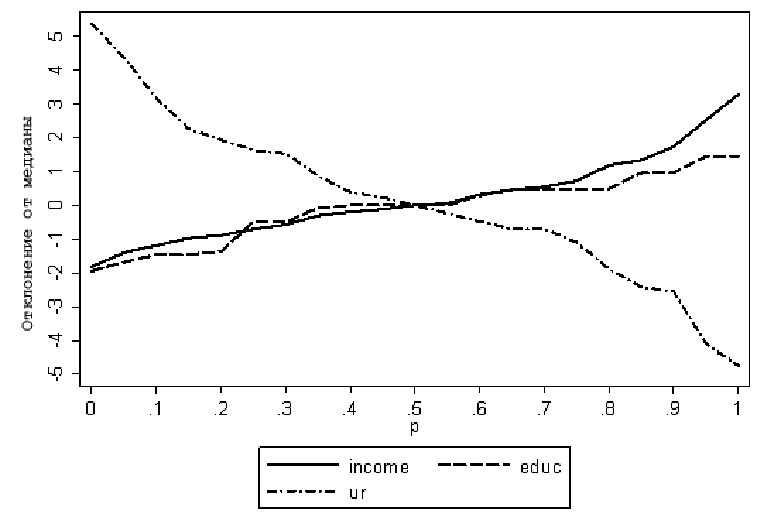
\includegraphics[width=12cm]{femalelabor.png}
	\caption{Название рисунка}\label{fig:femalelabor}
\end{figure} 

Квантильный размах вклада объясняющего признака отражён на этом графике как величина прироста или спада соответствующей линии между нужными квантилями. Такой график позволяет более полно представить себе важность объясняющих переменных. Например, из него видно, что доход и~длительность обучения имеют схожий по величине вклад в~переменную отклика. Вклад дохода имеет больший размах только за счёт нескольких штатов с~высоким уровнем благосостояния "--- об этом свидетельствует близость линий «educ» и~«income» на графике и~ускоренный рост линии «income» в~правой части (около девятой децили и~правее). 

Отметим, что линии на графике "--- результат сдвига и~пропорционального растяжения квантильных функций объясняющих признаков, потому они несут в~себе всю информацию о~частном распределении регрессоров, так как частное распределение однозначно задаётся функцией квантилей. Поэтому графики такого рода дают наглядную поддержку не только регрессионным оценкам, но и~описательной статистике.

{\bf Общий случай.} Рассмотренный подход к~измерению и~наглядному представлению вклада может быть применён и~для нелинейных зависимостей. Пусть объясняемая переменная связана с~набором регрессоров и~случайной составляющей следующим образом:
\begin{equation}\label{eq:1}
y = f(x_1,\ldots,x_{j-1},x_{j+1},\ldots, x_k, \epsilon) + g(x_j),
\end{equation}
где $f(), g()$ "--- функции, на которые мы не накладываем ограничений\footnote{Здесь можно порассуждать на тему «а~что если эти функции не могут быть случайными величинами», но ценность таких рассуждений сомнительна. В~любом случае, выборочные квантили будут существовать, даже если нет теоретических.}\fnnsp. Тогда мы можем оценить важность признака $x_j$ по квантильному размаху значений оценённой функции $g(x_j)$ в~имеющихся наблюдениях. При этом теряется возможность отразить направление связи "--- это, однако, не проблема способа измерения важности объясняющего признака, а~просто следствие того, что связь может иметь разные направления на разных участках значений объясняющей переменной. При этом в~уравнение регрессии признак может быть включён с~помощью нескольких переменных, например, линейным и~квадратичным членами, либо набором двоичных величин. Не возникает трудностей и~при анализе логарифмических зависимостей вида:
\begin{equation}\label{eq:2}
\ln y = f(x_1,\ldots,x_{j-1},x_{j+1},\ldots, x_k, \epsilon) + g(x_j).
\end{equation}
Отличие от предыдущего случая заключается в~том, что здесь можно измерить относительный вклад вместо абсолютного "--- оценить, {\it во сколько раз} изменяется величина отклика при изменениях признака $x_j$. Показателем важности признака будет квантильный коэффициент $\sfrac{\mathcal{Q}_G\left(\sfrac{1+\gamma}{2}\right)}{\mathcal{Q}_G\left(\sfrac{1-\gamma}{2}\right)}$ для величины $G = \exp(g(x_j))$. В~силу инвариантности квантилей к~монотонным преобразованиям этот коэффициент равен потенцированному квантильному размаху значений функции $g(x_j)$ "--- вклада признака $x_j$ в~логарифм переменной отклика. Рассмотрим этот случай на ещё одном примере из области статистических исследований рынка труда.

\subsubsection*{{\it Пример 2. Уравнение заработной платы}}

По индивидуальным данным\footnote{взятым отсюда: \url{http://www.wiley.com/legacy/wileychi/verbeek2ed/datasets.html} "--- здесь выложены файлы с~данными для примеров из учебника М. Вербика по эконометрике.} обследования рабочих в~Бельгии (1994 г.) оценивалось уравнение:
\[\ln W_i = \beta_1 + \beta_2Male_i + \beta_3Exp_i + \beta_4Exp_i^2+ \beta_5E2_i + \beta_6E3_i + \beta_7E4_i+ \beta_8E5_i + \epsilon_i,\]

где $W_i$ "--- заработная плата $i$-го рабочего в~выборке (бельгийские франки),

$Male_i$ "--- пол (1--- мужчина, 0 --- женщина),

$Exp_i$ "--- опыт работы (годы),

$E2_i,\ldots, E5_i$ "--- дамми"=переменные для уровня образования ($E5=1$ для наивысшего уровня, базовая категория "--- самый низкий уровень образования).

\begin{table}[ht]
	\begin{center}
		\begin{tabular}{cccccc}
			\hline
			\multirow{4}{*}{Признак}& \multirow{4}{*}{Коэффициент}& \multirow{4}{*}{Оценка} &  & Вклад, & Вклад,\\
			&&& Потенцированная & относительный & квантильный\\
			&&& оценка & размах\tablefootnote{Под относительным размахом здесь понимается отношение наибольшего значения к~наименьшему.} & коэффициент\\
			&&&& & $\sfrac{Q(0.95)}{Q(0.05)}$\\
			\hline
			Пол& $\beta_2$& 0.115& 1.122& 1.122& 1.122\\
			\multirow{2}{*}{Опыт работы}& $\beta_3$& 0.034 & 1.035&\multirow{2}{*}{1.821} &\multirow{2}{*}{1.700}\\
			&$\beta_4$& -0.0005& 0.9995& &\\
			\multirow{4}{*}{Образование} & $\beta_5$& 0.141& 1.152& \multirow{4}{*}{1.898}&\multirow{4}{*}{1.898}\\
			&$\beta_6$& 0.308& 1.362&&\\
			&$\beta_7$& 0.481& 1.618&&\\
			&$\beta_8$& 0.641& 1.898&&\\
			\hline
		\end{tabular}
	\end{center}
\end{table}

Отметим, что коэффициенты $\beta_3, \beta_4$ практически не поддаются интерпретации (остальные интерпретируемы в~потенцированном виде) и~что ни один из стандартизированных или полустандартизованных коэффициентов не имеет смысла. Для двоичных переменных бессмысленно рассматривать изменение на одно стандартное отклонение, для переменных $Exp$ и~$Exp^2$ не может идти речь о~«прочих равных условиях» "--- абсурдно рассматривать изменение одной из них при постоянстве другой. Тем не менее, оценки уравнения регрессии могут быть сопровождены осмысленными мерами вкладов каждого из трёх признаков.

Согласно полученным оценкам, наиболее существенный вклад в~уровень зарплаты приходится на уровень образования: различия по этому признаку объясняют расхождение заработной платы в~1.898 раз. Схожую по величине роль играет и~общий стаж. Если бы наблюдения в~выборке отличались только по числу отработанных лет, то модельные значения заработной платы отличались бы не более чем в~1.821 раз во всей выборке и~не более чем в 1.7 раза в~средних 90\% наблюдений. 

Наглядное изображение важности вклада признаков даёт график отношения квантилей вкладов к~медианному вкладу, на котором по горизонтальной оси откладывается порядок квантили $p$, а~по вертикальной "--- величина $\sfrac{\mathcal{Q}_G(p)}{\mathcal{Q}_G(0.5)}$:

\begin{figure}[htbp]
	\centering
	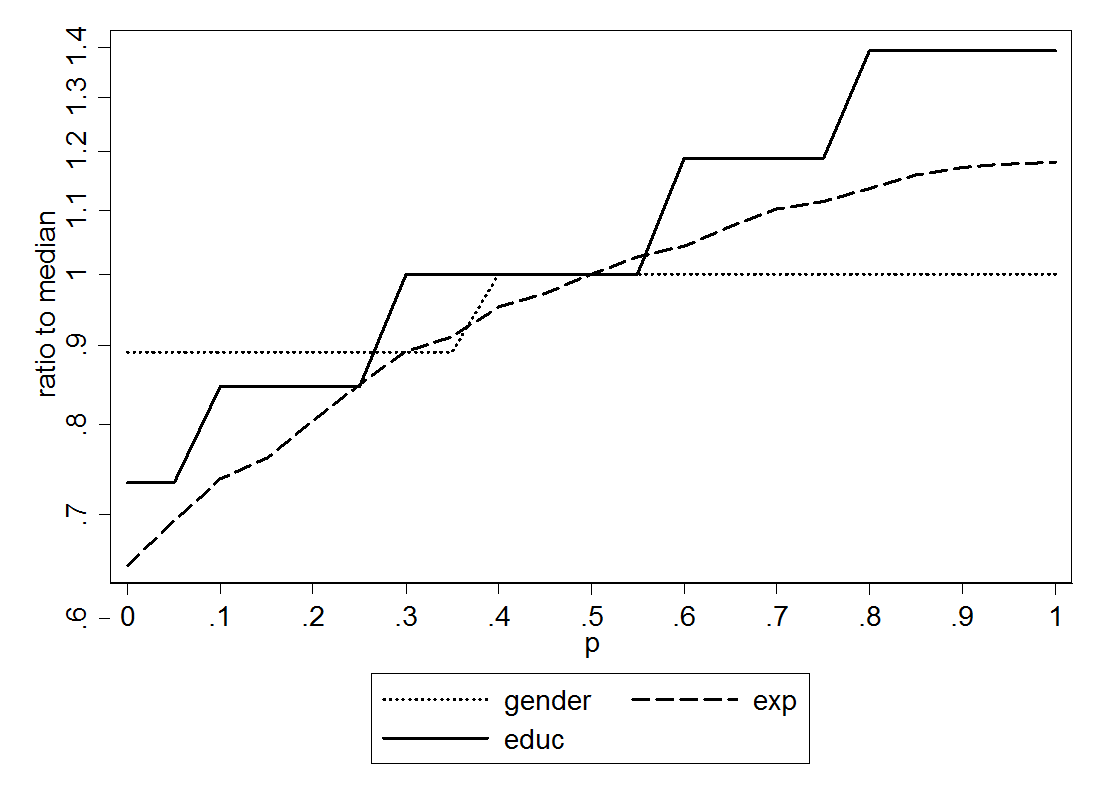
\includegraphics[width=12cm]{wageeq.png}
	\caption{Название рисунка}\label{fig:wageeq}
\end{figure} 

Так как по вертикальной оси откладывается отношение, график предпочтительно изображать в~логарифмической шкале. Отражая схожий во величине вклад образования и~опыта работы, график подчёркивает асимметричность: при прочих равных условиях у~людей без опыта работы заработная плата отклоняется от медианной сильнее, чем у~наиболее опытных.

{\bf Критика, ответ и~опять критика.} В~отношении предложенного способа измерения практической важности вклада можно выразить ту же критику, что неоднократно высказывалась против стандартизованных коэффициентов: оговорка «при прочих равных» выглядит слишком отдаляющей от действительности. Для экономических приложений естественна связь между объясняющими переменными: изменению одной из них должны сопутствовать изменения других. Само по себе такое замечание неоспоримо, однако стоит иметь в~виду, что цель множественного регрессионного анализа "--- именно выделение связей, изолированных от постороннего влияния. То есть, критика относится скорее к~самому подходу, при котором основой анализа становится одна модель множественной регрессии без попыток изучения опосредованных связей (mediation). При желании «освободить» какой-либо из регрессоров можно просто исключить его из модели и~сравнить результаты, полученные до и~после исключения. Это только увеличит объём возможно полезных сведений в~копилке исследователя. Правда, чем больше этих сведений, тем сложнее их свести к~однозначному выводу.

{\bf Возможные расширения применимости.} Формулы \eqref{eq:1} и~\eqref{eq:2} не стоит рассматривать как строгие границы, вне которых для измерения важности объясняющих переменных придётся искать существенно иные подходы. Заметим, что в~качестве объясняемой величины $y$ не обязательно должен фигурировать именно статистический признак "--- это может быть какая-либо интерпретируемая характеристика распределения этого признака, например шансы (odds) какого-либо события при моделировании бинарного выбора или функция риска (hazard function) при моделировании времени жизни.

Дополнительные возможности для иллюстрации предлагаемого подхода даёт использование панельных данных: разбиение вклада признаков на межгрупповой (between) и~внутригрупповой (within) разброс, сравнение вклада наблюдаемой разнородности (отдельных переменных или всей совокупности регрессоров) с~ненаблюдаемой (индивидуальным эффектом).

{\bf Пара абзацев в~конце.} Ещё раз отмечу: в~статье речь идёт о~таком аспекте практической значимости, как вклад разброса объясняющего признака в~разброс регрессанта при прочих равных условиях («dispersion importance», говоря словами К.Эйкена – см. (Achen, 1982, стр. 73-77)). Исследование практической значимости, конечно, не сводится только к~этому аспекту. Это вообще не то, что можно было бы полностью формализовать и~свести к~математическим мерам. Моя цель скромнее "--- предложить такой способ численно и~графически описать связь между признаками, который был бы полезным подспорьем при выяснении практической значимости.

Квантили "--- не единственный способ получить интерпретируемые меры разброса. Можно опираться на среднее абсолютное отклонение величины от своего среднего или медианы, хотя я~не знаю, как на их основании построить столь же информативные графики. Предлагаю читателю самому обдумать соответствующие характеристики вклада объясняющих переменных.

\medskip
\textit{Основа этого текста "--- доклады на семинаре кафедры математической экономики и~эконометрики и~семинаре департамента прикладной экономики НИУ ВШЭ, сделанные в~2013 году. Автор благодарит Г.Г.~Канторовича, Э.Б.~Ершова, Б.Б.~ Демешева и~А.А.~Пересецкого за обсуждение.}


\printbibliography	
	
\end{document}